\chapter{Experimental Evaluation}
\label{chapter:expRsults}
In this Chapter, we detail the experimental results obtained during different phases of the project. First, we present the information about the study that allowed us to pick the most suitable algorithm for the recommender system. Then, we describe the performance tests that were made in order to establish service usage limits.

\section{Recommender System}
\label{subsec:expRsults}
In this Subsection, we present the experimental results regarding the evaluation of different recommender systems. To provide reliable evaluation results, we have implemented a few variations of the recommender systems using different algorithms, provided by the Mahout library. We analyse the performance and the quality aspects of the produced recommendations, which have helped to choose the best algorithm for our needs.\\
\\
For the evaluation purpose we have used the MovieLens~\cite{movieLens} datasets provided by GroupLens~\cite{gourpLens} research. MovieLens is a movie recommender site used to study recommendation engines. We have chosen this dataset due to the equality of the rating scale chosen for the GuideMe service.\\
\\
For the recommender system evaluation, we have used the datasets illustrated on Table~\ref{tab:DatasetSize}.
\begin{center}
\begin{table}
	\centering
    \caption{MovieLens datasets used for evaluation.}
    \label{tab:DatasetSize}
    \begin{tabular}{c}
	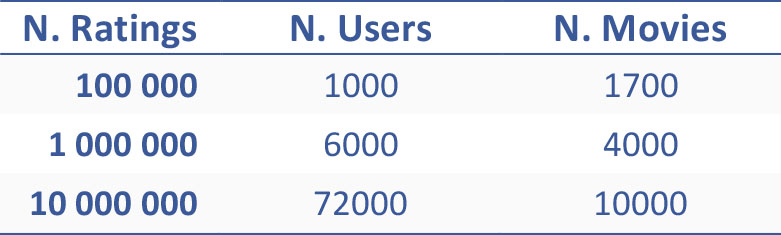
\includegraphics[height=2cm]{./images/tables/table_moviles_dataset_distribution.jpg}    
    \end{tabular}
    \end{table}
\end{center}
%%%%%%%%%%%%%%%%%%
In order to measure the accuracy of the different algorithms, we have used the \gls{mae} metric. Absolute error value is computed for each rating-prediction pair $<p_i, p_q>$, then is computed the average. Formally, 
\begin{equation}
MAE=\frac{\sum_{i=1}^{n} | p_i - p_q|}{n}
\end{equation}
which refers to the deviation (in a range $0 \le MAE \le 1$) of the recommendations from their user-specified values~\cite{ibCollabrativeVSGK}. The lower the \gls{mae}, the more accurately the recommendation engine predicts user ratings. For most of the evaluations, we divided the datasets shown on Table~\ref{tab:DatasetSize} in two different sets, the training set which holds around $80\%$ of data and the test set with the remaining $20\%$. In other evaluation scenarios, we indicate the distribution of data between the training and the test datasets.\\
\\
To correctly measure the \gls{mae} value, the initial idea was to use the K-Fold Cross Validation\footnote{K-Fold Cross Validation is a model validation technique. It is commonly used in environments where the goal is prediction, and one wants to estimate how accurately a predictive model will perform in practice. Consists in dividing the dataset into $K$ sub-samples, where $k-1$ sub-samples are used as training data and a single sample is retained for validation. The validation process is repeated $K$ times, with each of the $K$ sub-samples used exactly once as the validation data.} method~\cite{Duda_Book}. It was not possible to apply this technique, since the latest version of the Mahout library (v0.7) does not provide any hooks for the implementation of this evaluation methodology. There is no way to divide the dataset into the training and the test sets and repeat the recommendation process alternating between $K$ sub-samples. Instead of K-Fold Cross Validation, to ensure more accurate \gls{mae} results, each algorithm was executed 5 times, being the evaluation value the average of those executions.\\
\\
For the following evaluations, we have chosen four different algorithms, Slope One, IB with Euclidean Distance, IB with Log Likelihood, and IB with uncentered cosine. The evaluation of the performance of these algorithms is illustrated on Figure~\ref{fig:chartEvalPerformance} where the lowest \gls{mae} value is achieved by the Slope One algorithm. With the growing of the dataset, the presented algorithms become more accurate with the recommendations.\\
%%%%%%%%%%%%%%%%%%
\begin{figure}[h!]
 \centering
   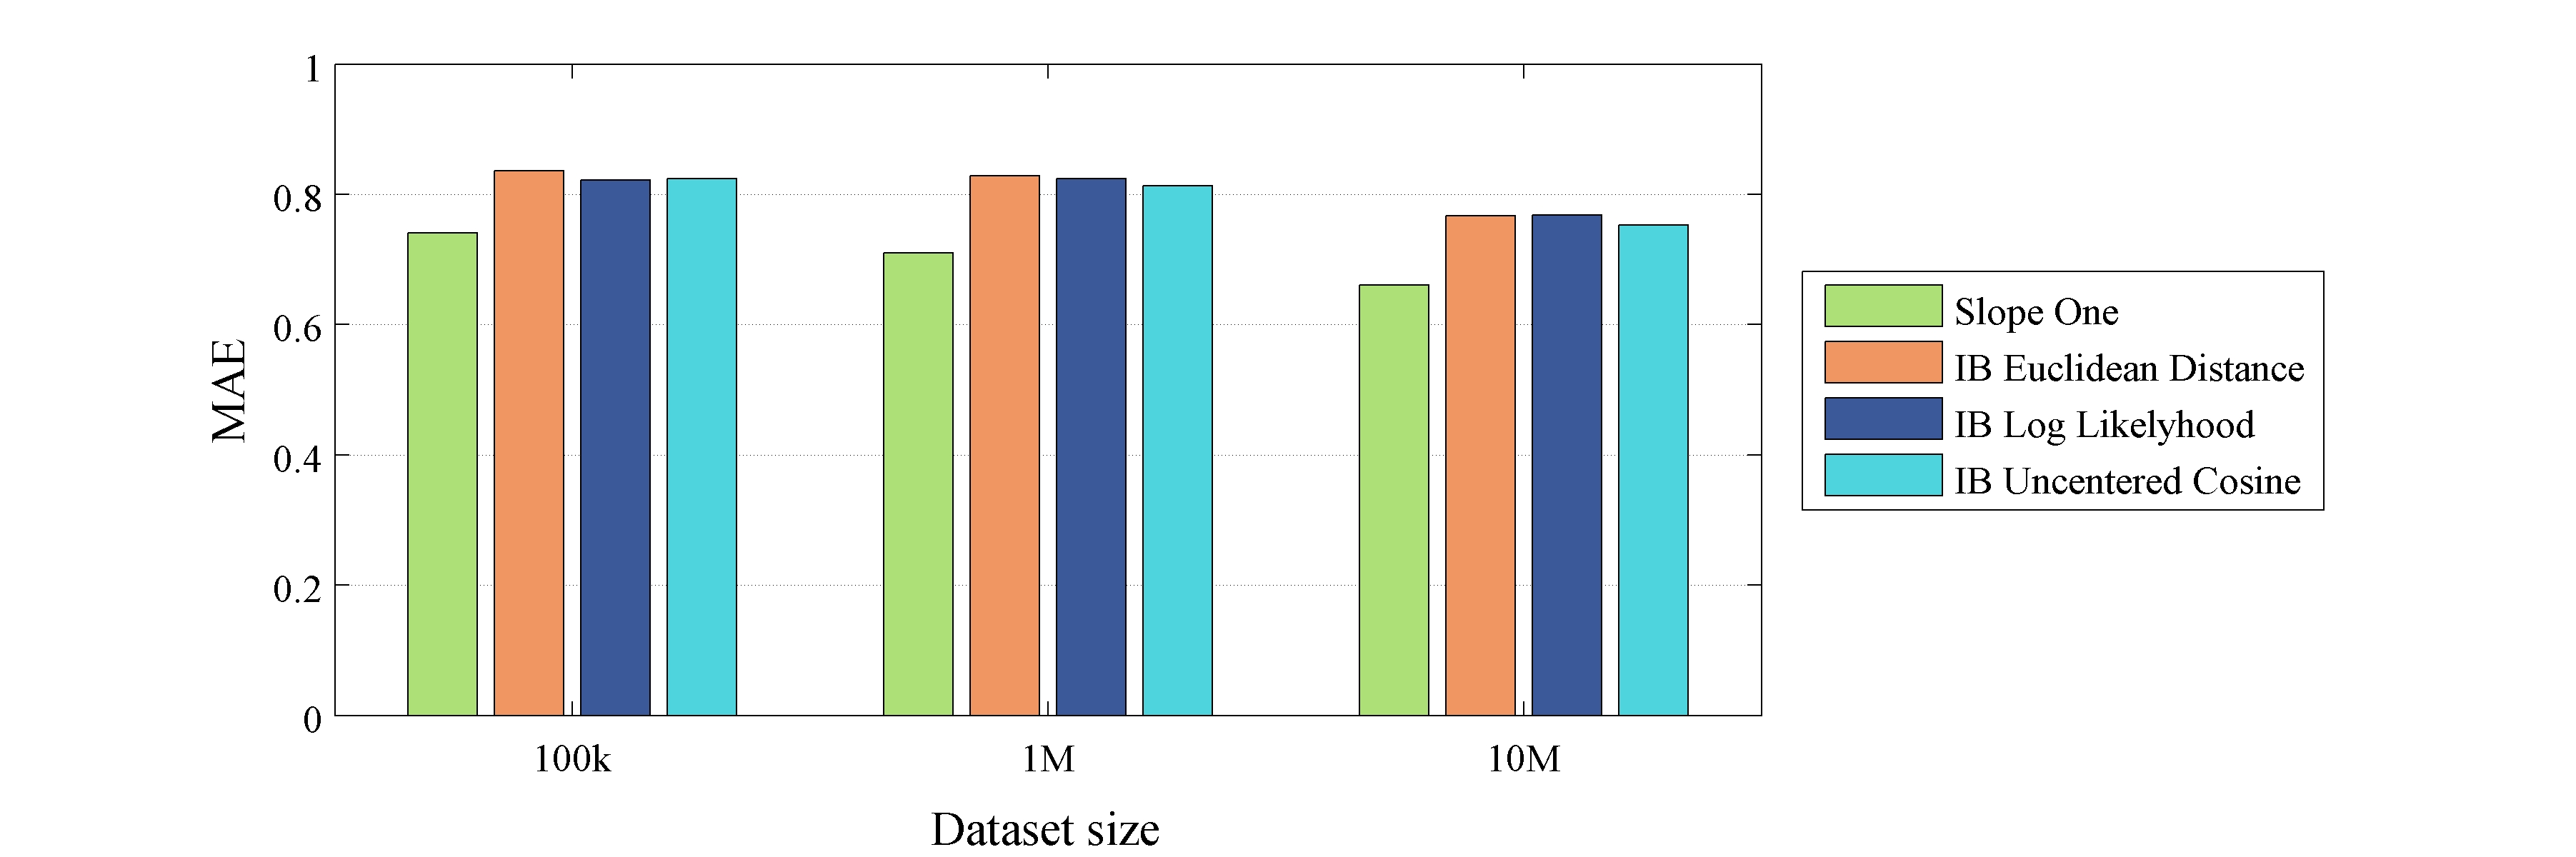
\includegraphics[width=13cm]{./images/charts/charts_eval_alg_performance.jpg}
   \caption{Performance of different recommender algorithms.}
   \label{fig:chartEvalPerformance}
\end{figure}\\
%%%%%%%%%%%%%%%%%%
On Figure~\ref{fig:chartExecutionTime} we show the execution time of the analysed algorithms. The Slope One requires a lot of physical memory in order to compute the data model which then is used for recommendations, but it presents benefits in terms of performance when compared with other implementations.\\
\begin{figure}[h!]
 \centering
   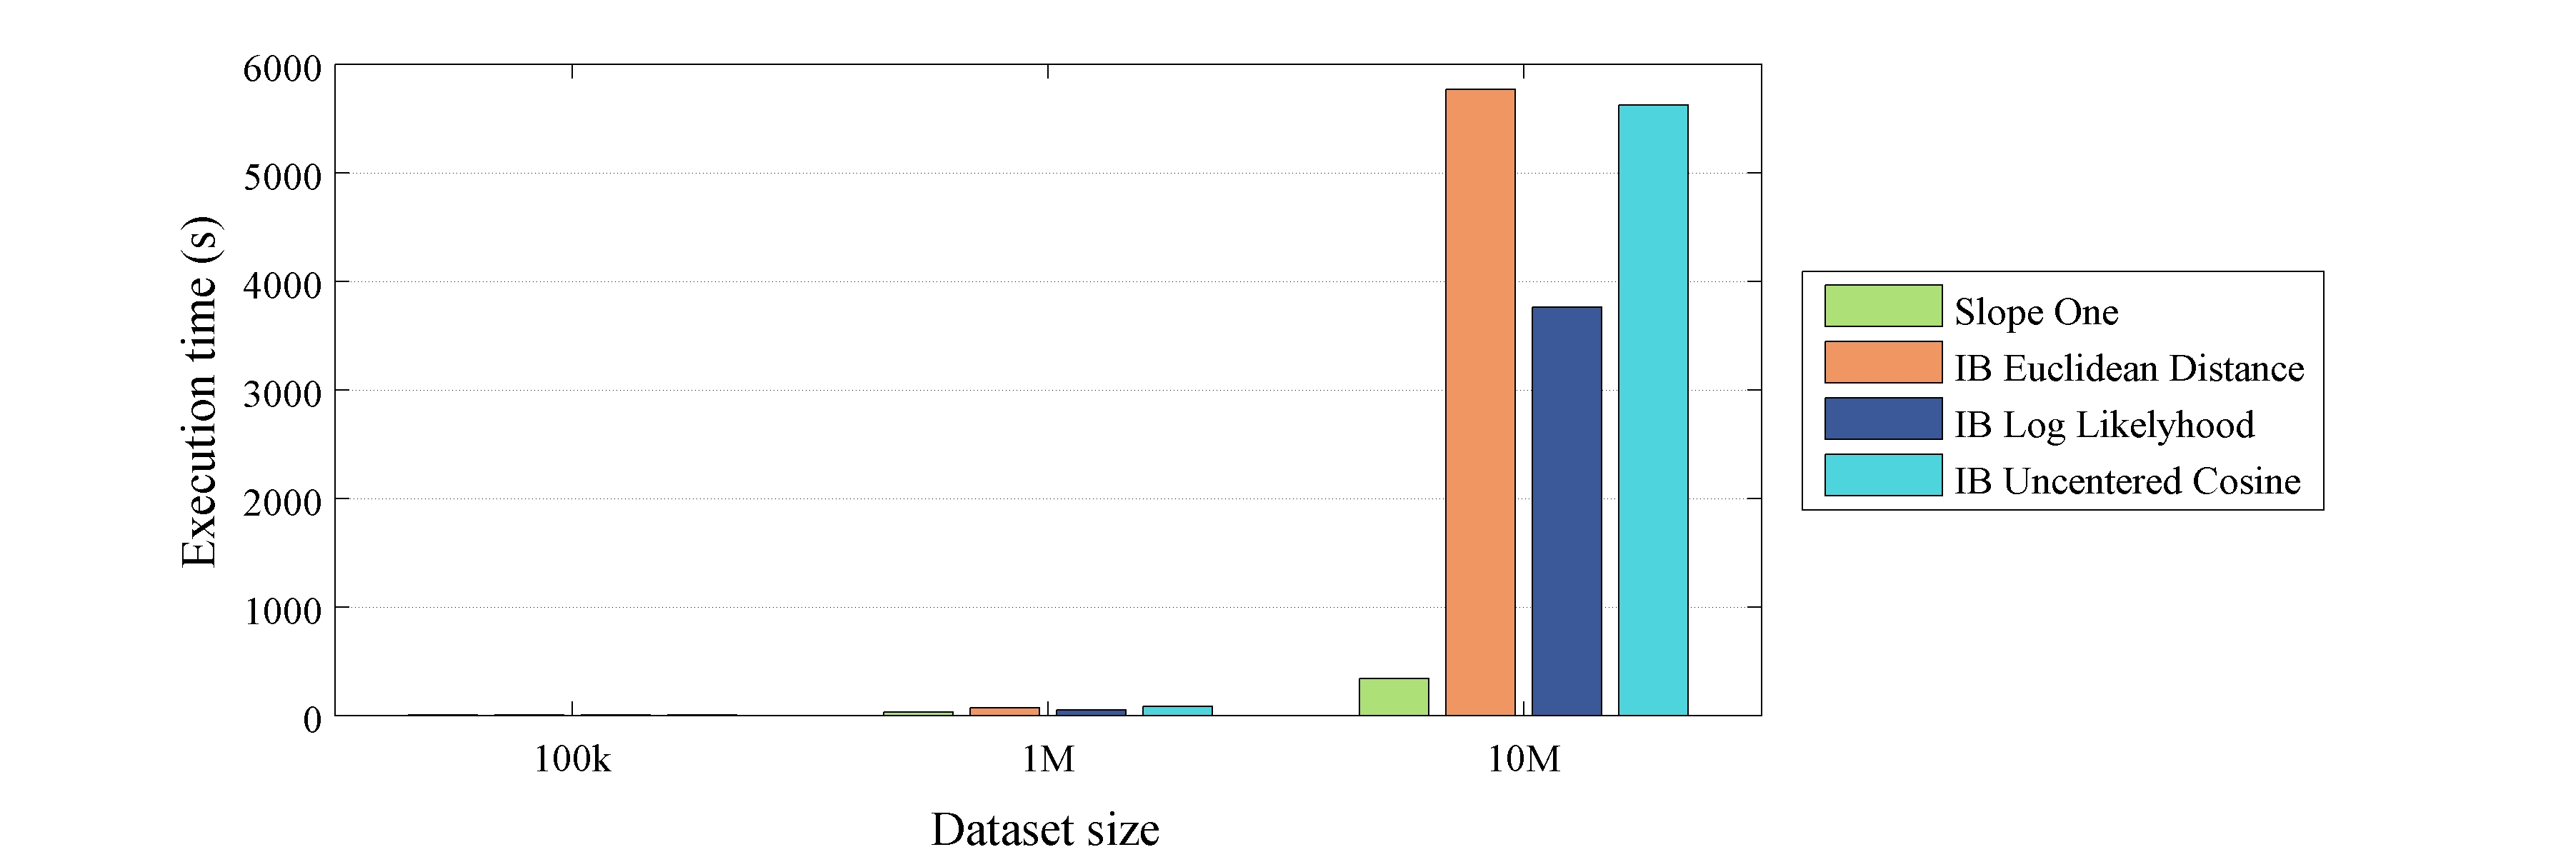
\includegraphics[width=13cm]{./images/charts/charts_eval_alg_execution_time.jpg}
   \caption{Evaluation of the execution time.}
   \label{fig:chartExecutionTime}
\end{figure}\\
%%%%%%%%%%%%%%%%%%
The presented analysis allowed us to make an appropriate choice of the algorithm for our recommender system. The forthcoming evaluations are based on variations of the Slope One algorithm. In order to minimize the memory consumption, we calibrate the algorithm with different sizes for the diff storage\footnote{Diff storage contains a precomputed average differences in preference values between all pairs of items. The number of diffs is configurable and the algorithm will try to keep the most useful diffs. Most useful here means those diffs between a pair of items that turn up most often together in the list of items associated with a user~\cite{mahoutInAction}.}. For the following evaluations we are considering the unlimited diff storage, diff storage with 500000, and 100000 entries. On Figure~\ref{fig:chartSlopeOneModeSize}, we show that the \gls{mae} value is lower for the unlimited diff storage. The results are satisfying when the diff storage is limited to 500000 entries, thus minimizing memory consumption.\\
%Main info sobre diff size está no livro do Mahout (Página 75).
\begin{figure}[h!]
 \centering
   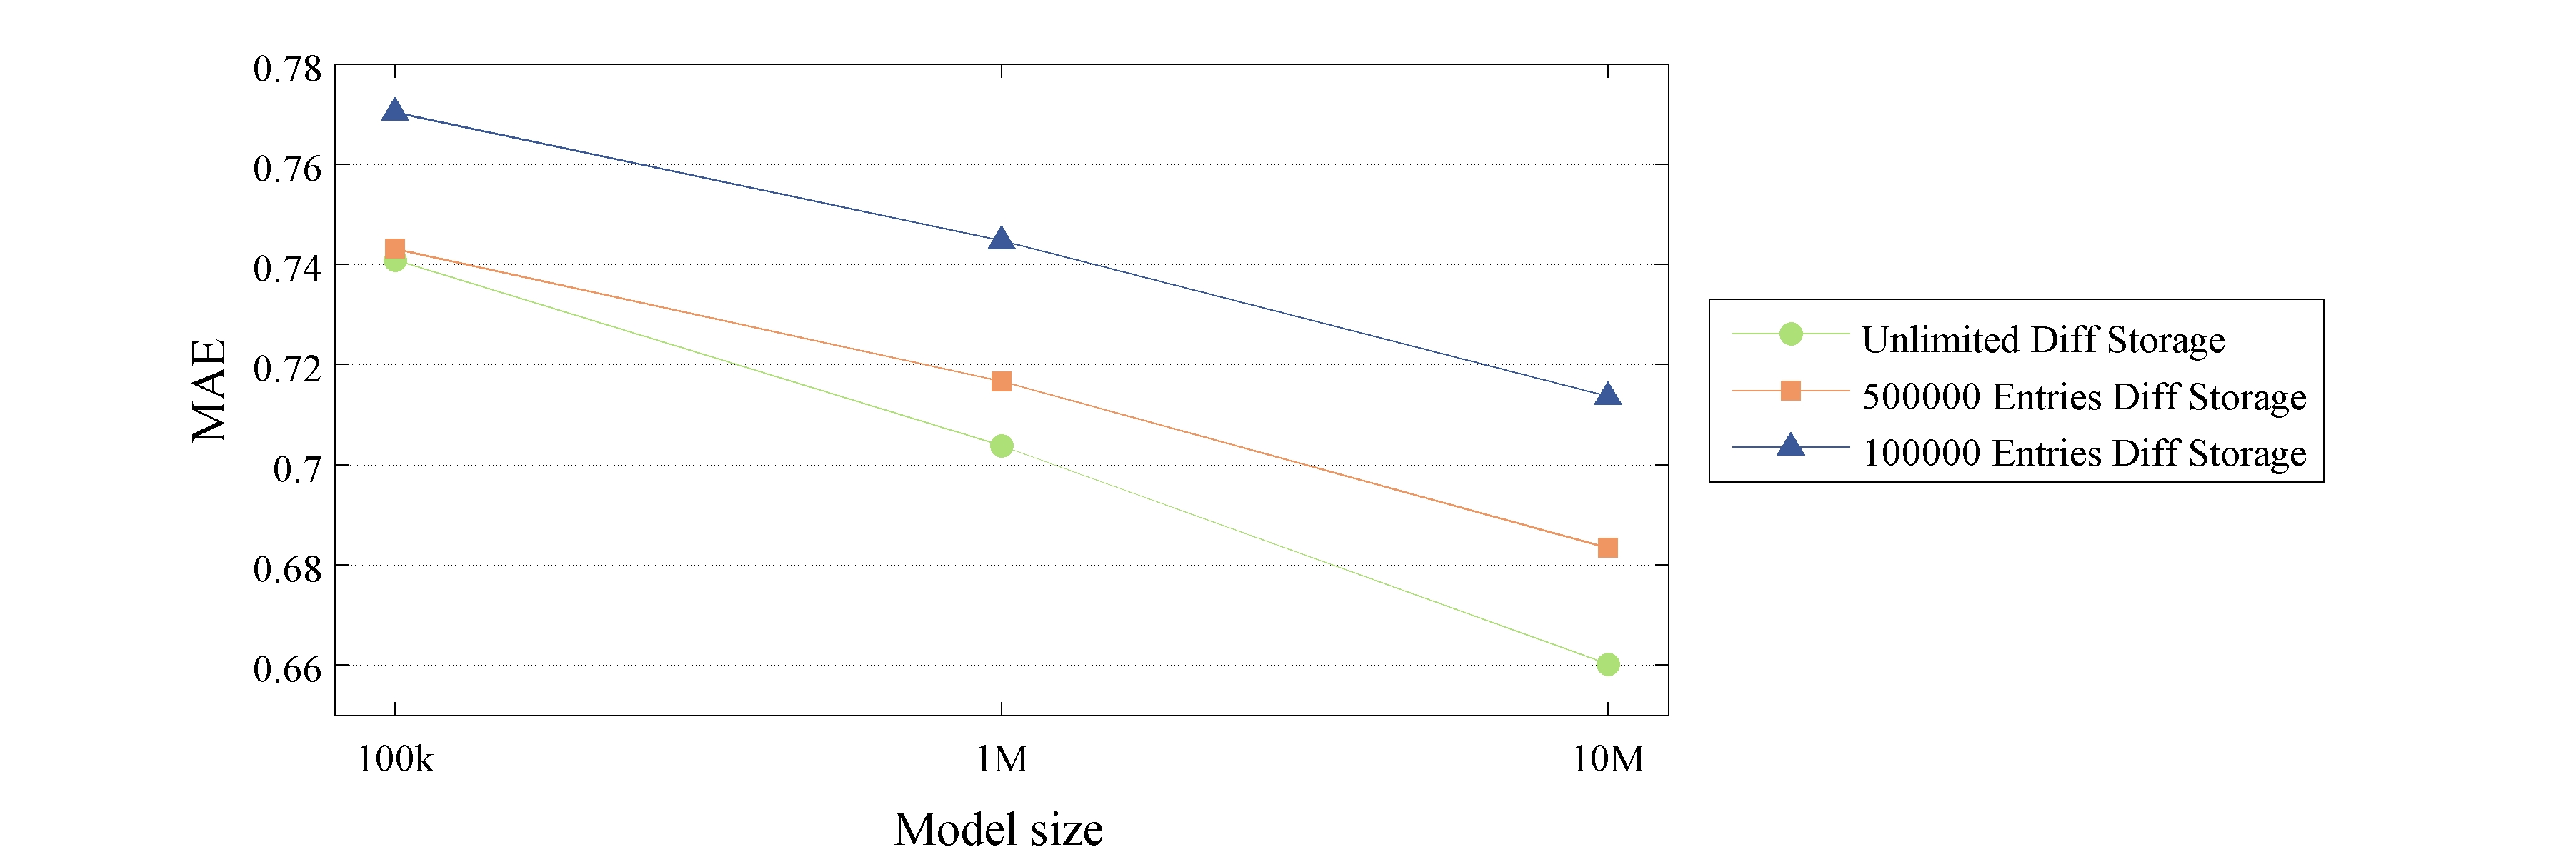
\includegraphics[width=13cm]{./images/charts/charts_eval_alg_slopone_model_size.jpg}
   \caption{Sensitivity of the diff storage size for the Slope One algorithm.}
   \label{fig:chartSlopeOneModeSize}
\end{figure}\\
%%%%%%%%%%%%%%%%%%
Some evaluations were made by varying the percentage of the training and the test sets as illustrated on Figure~\ref{fig:chartTrainingTestSet}. We have concluded that a larger dataset implies better recommendation results. By using the diff storage limited to 500000 entries, the \gls{mae} value for the training set of $80\%$ is around $0.7$, better than the other algorithms reported on Figure~\ref{fig:chartEvalPerformance}.\\
\begin{figure}[h!]
 \centering
   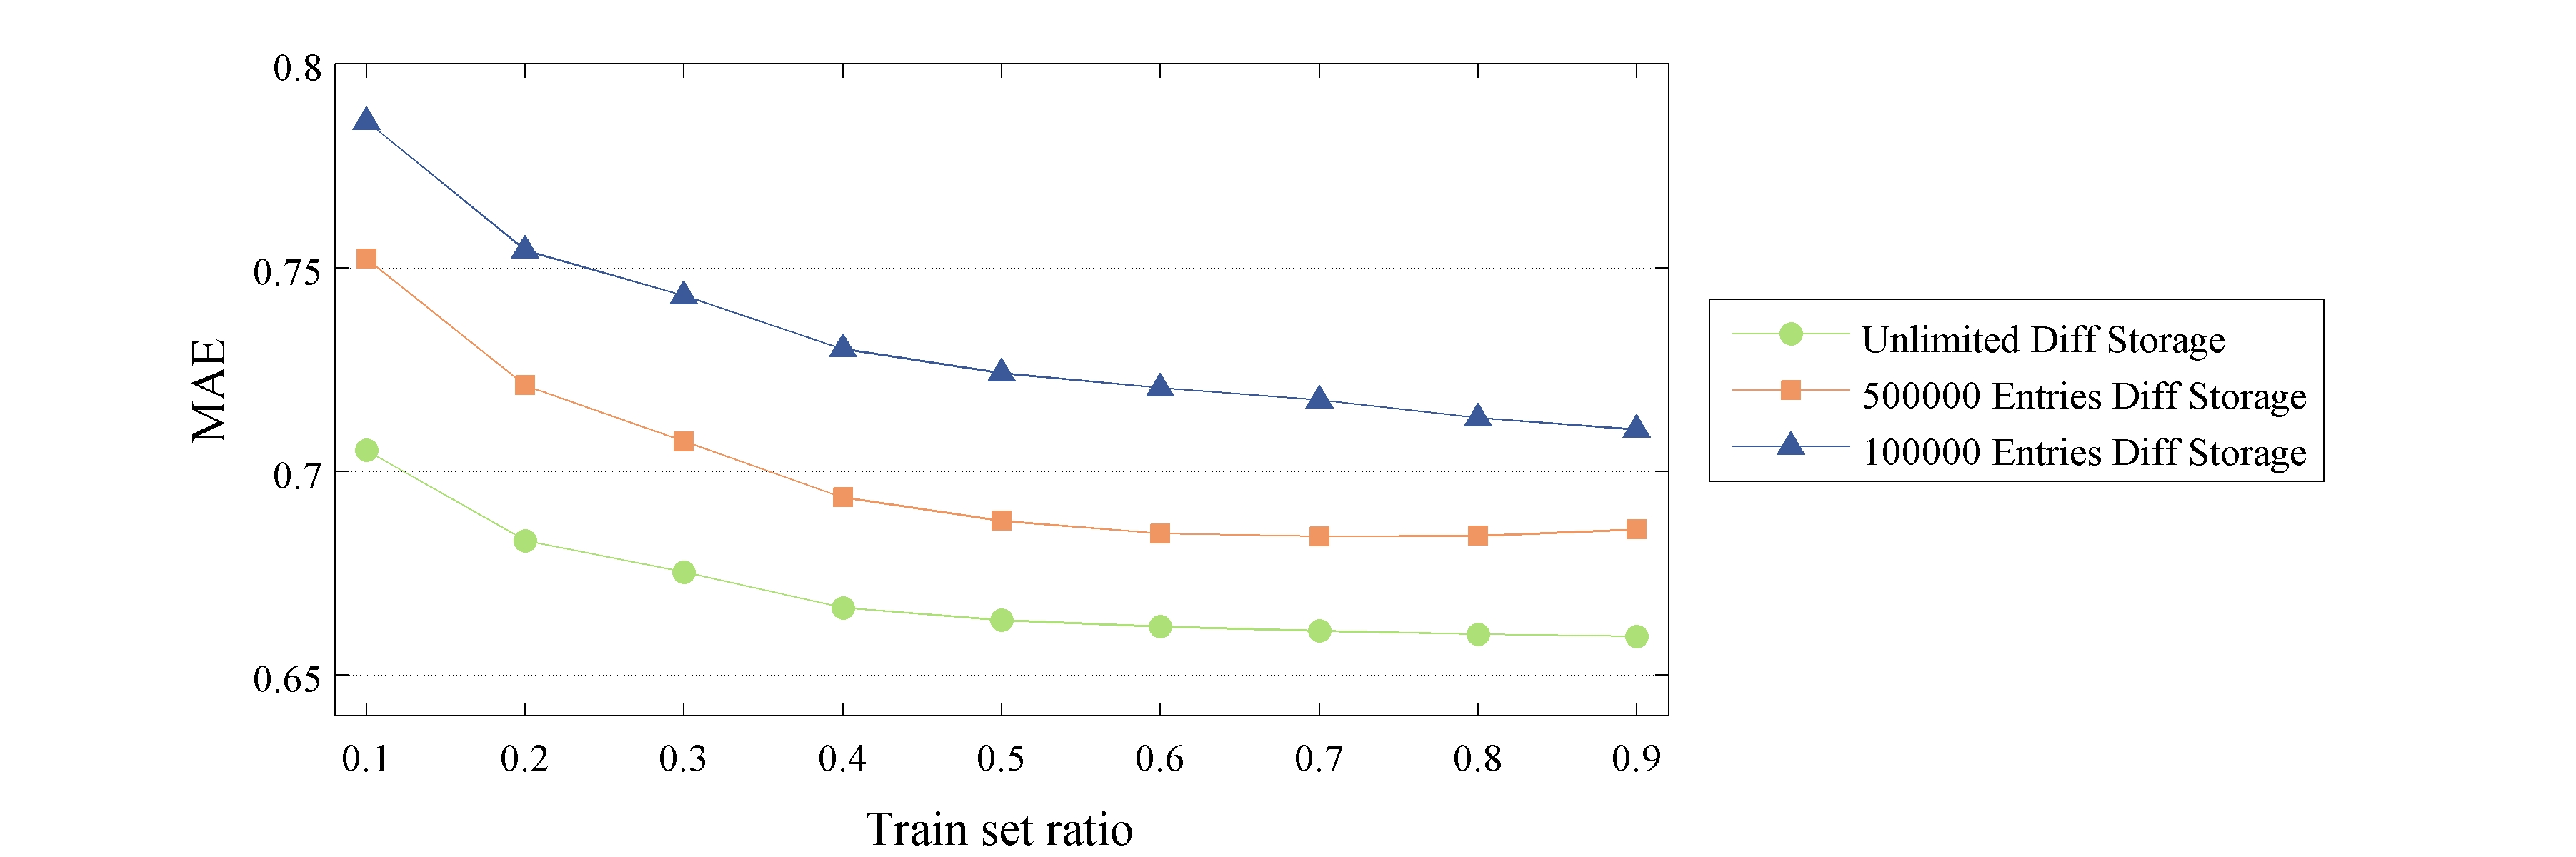
\includegraphics[width=13cm]{./images/charts/charts_eval_alg_slopone_dataset_ration.jpg}
   \caption{Variation of the dataset ratio for the Slope One algorithm.}
   \label{fig:chartTrainingTestSet}
\end{figure}\\
%%%%%%%%%%%%%%%%%%
These evaluations allowed us to choose the more suitable recommendation algorithm for our dataset, being our recommendation engine implemented with the Slope One algorithm configured with unlimited diff storage. In the future, with the grow of the dataset, we will limit the algorithm to 500000 diff storage entries.

\section{Load Tests}
\label{subsec:loadTests}
In this Section, we detail the utility of the performed load tests, which allowed to evaluate the performance of the implemented service and detect issues that were affecting negatively its functionalities. All the tests are made to the REST API, deployed on Amazon EC2~\cite{amazonEC2} instance with specification described in Table~\ref{tab:ec2Specs}.
\begin{center}
\begin{table}
	\centering
    \caption{Amazon EC2 instance specification.}
    \label{tab:ec2Specs}
    \begin{tabular}{c}
	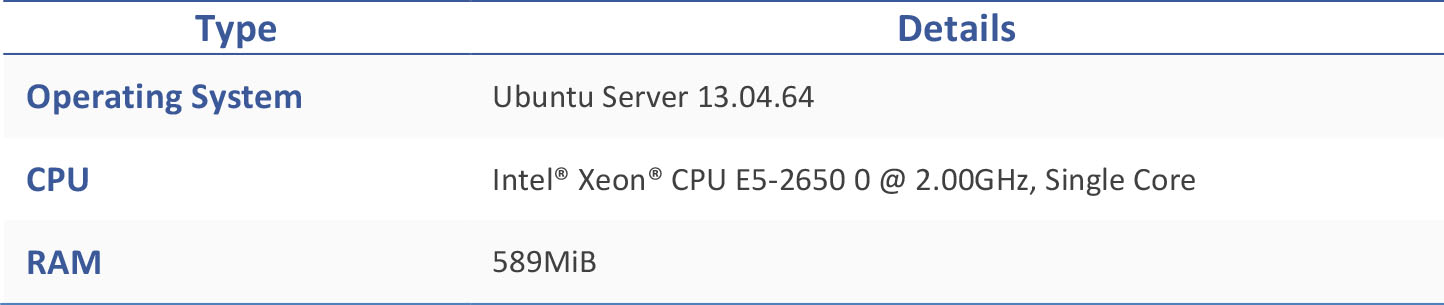
\includegraphics[width=11cm]{./images/tables/table_server_specs.jpg}
    \end{tabular}
    \end{table}
\end{center}
We have used the Gatling Stress Tool~\cite{gatling} to perform the load tests. The tests are named as simulations and are written in Scala. Each simulation is composed by a scenario, which represent users' behaviours, composed by one or multiple requests. To achieve reliable feedback, we have created a test scenario based on eight different requests, as detailed in Table~\ref{tab:testcase}. 
\begin{center}
\begin{table}
	\centering
    \caption{Requests for the testing test case.}
    \label{tab:testcase}
    \begin{tabular}{c}
	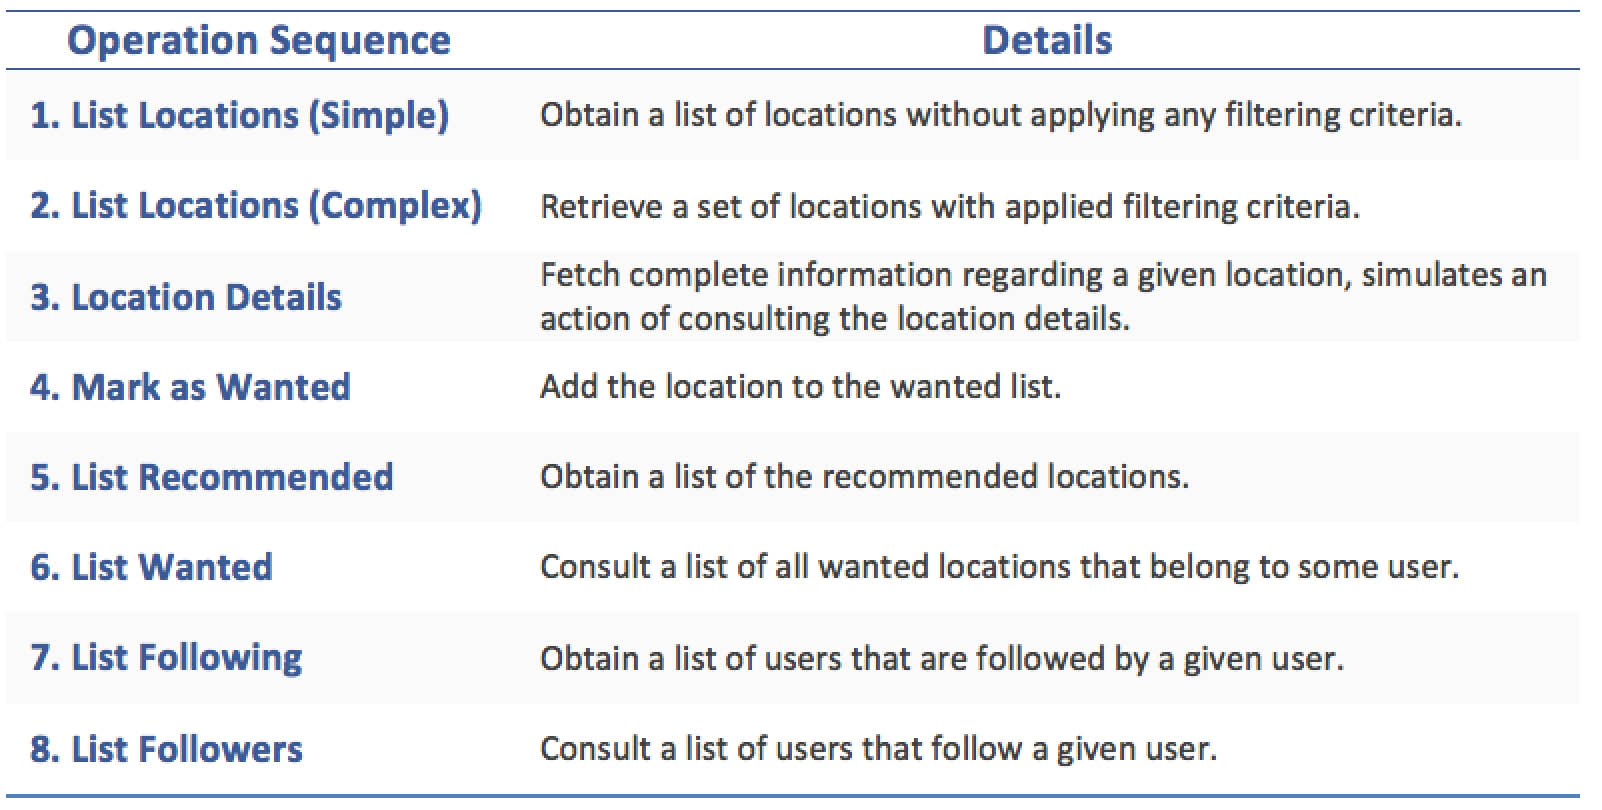
\includegraphics[width=11cm]{./images/tables/table_load_testcase.jpg}
    \end{tabular}
    \end{table}
\end{center}
The created scenario was executed several times varying the number of users within range $\{1, 2, 5, 10, 20, 50, 100, 200\}$ where each user performs the eight requests, described in Table~\ref{tab:testcase}. Two different metrics were extracted from the execution of the scenario, one representing the number of the requests per second and other referring to the average request execution time. Figure~\ref{fig:evalMaxRequests} illustrates the relation between the number of users and the number of requests executed per second. The performance of the current scenario becomes slower when it is executed by more than 200 users.\\
%%
\begin{figure}[h!]
 \centering
   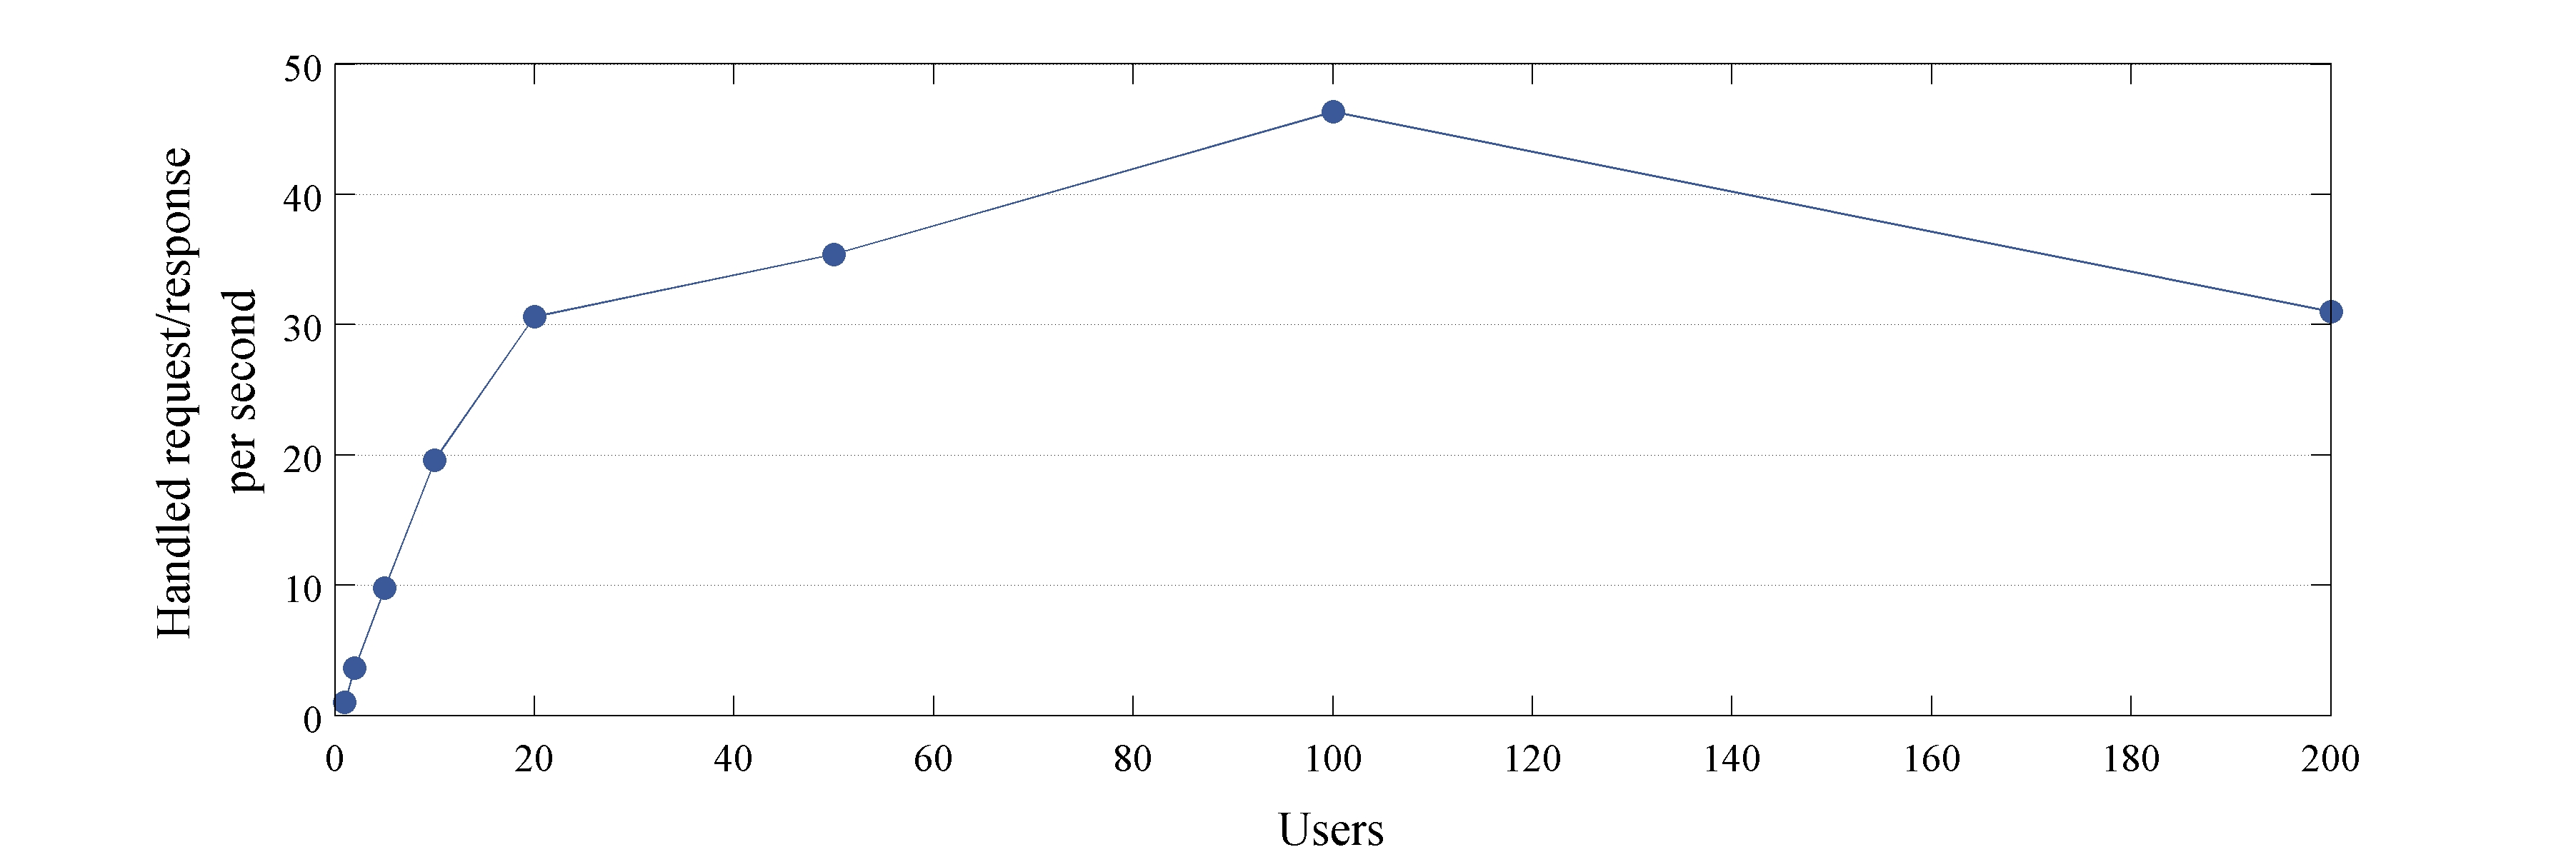
\includegraphics[width=13cm]{./images/charts/charts_eval_load_test_requests_per_second.jpg}
   \caption{Evaluation of the maximum number of the requests per second.}
   \label{fig:evalMaxRequests}
\end{figure}\\
%%
Figure~\ref{fig:avgRequestTime} shows the average request/response duration  when the operations are performed by varied number of users. The system handles well around 100 users, but it becomes slower with increase of the users per request.\\\\
%%
\begin{figure}[h!]
 \centering
   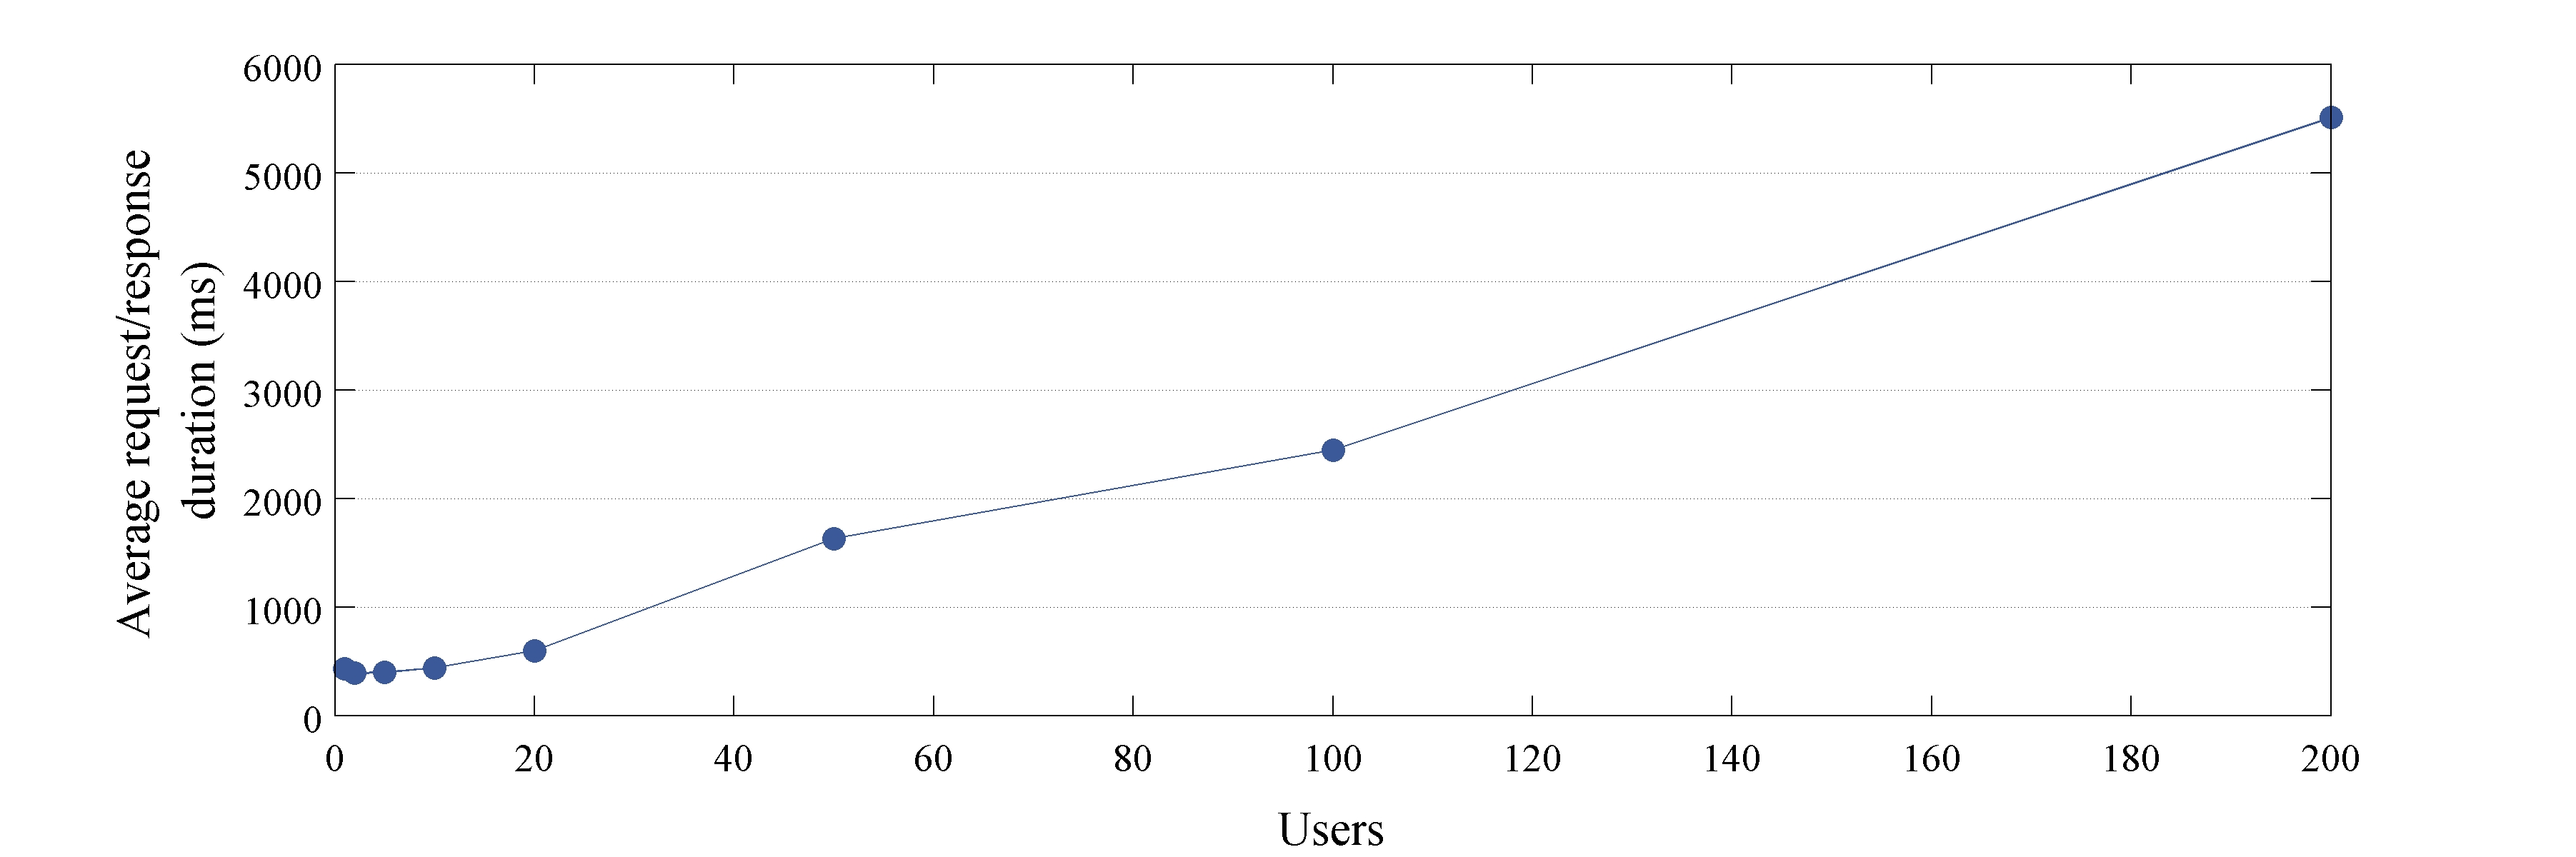
\includegraphics[width=13cm]{./images/charts/charts_eval_load_test_average_request_duration.jpg}
   \caption{Evaluation of the average request time.}
   \label{fig:avgRequestTime}
\end{figure}\\
%%
When the load tests were performed by the first time, those have helped to detect the database connection leaks. The life cycle of the connection was not correctly managed within DAO, which was surpassing periodically the maximum number of allowed database connections.\\
\\
These created tests not only helped to evaluate the performance of the system, but also to correct the critical bugs that have emerged during this phase.

\section{Usability Evaluation}
\label{subsec:usabilityEvaluation}
In this Section, we describe the usability evaluation process based on a survey. We begin by introducing the organization of the questionnaire and then we describe the statistical data regarding some of the questions posed to the users.\\
\\
In order to evaluate the usability of the developed application, we have collected the feedback from 30 users which have answered to a survey included in Appendix~\ref{sec:survey}. The survey is divided into four main categories, the general information where we collected the user’s gender and age range, followed by a set of questions related to user’s experience with mobile applications. The third section of the survey is composed by questions regarding the specific screens of the applications, where the user can rate the usefulness and attractiveness of the designed application. In the fourth section we ask the user if he/she would install the application in the future and optionally to leave some notes that may improve or enrich the application.\\
\\
Users have started by fill in the first two sections of the questionnaire. After, they were provided with the iOS device running the application and a maximum of 5 minutes to interact with it. No help were given during that time. Finally, they were asked to fill the third and fourth sections of the questionnaire describing their opinion and impressions regarding the application.\\
\\
Most of the users have liked the implemented set of features and the overall design of the application. Below, we present some statistical data that supports this statement. Figure~\ref{fig:usabilityOverall} shows the distribution of the ratings that people have given to classify the appearance and content organization in the different screens. The used rating scale is between one (unattractive and difficult to use) and five (attractive and easy to use).\\
%%%%%%%%%%%%
\begin{figure}[h!]
 \centering
   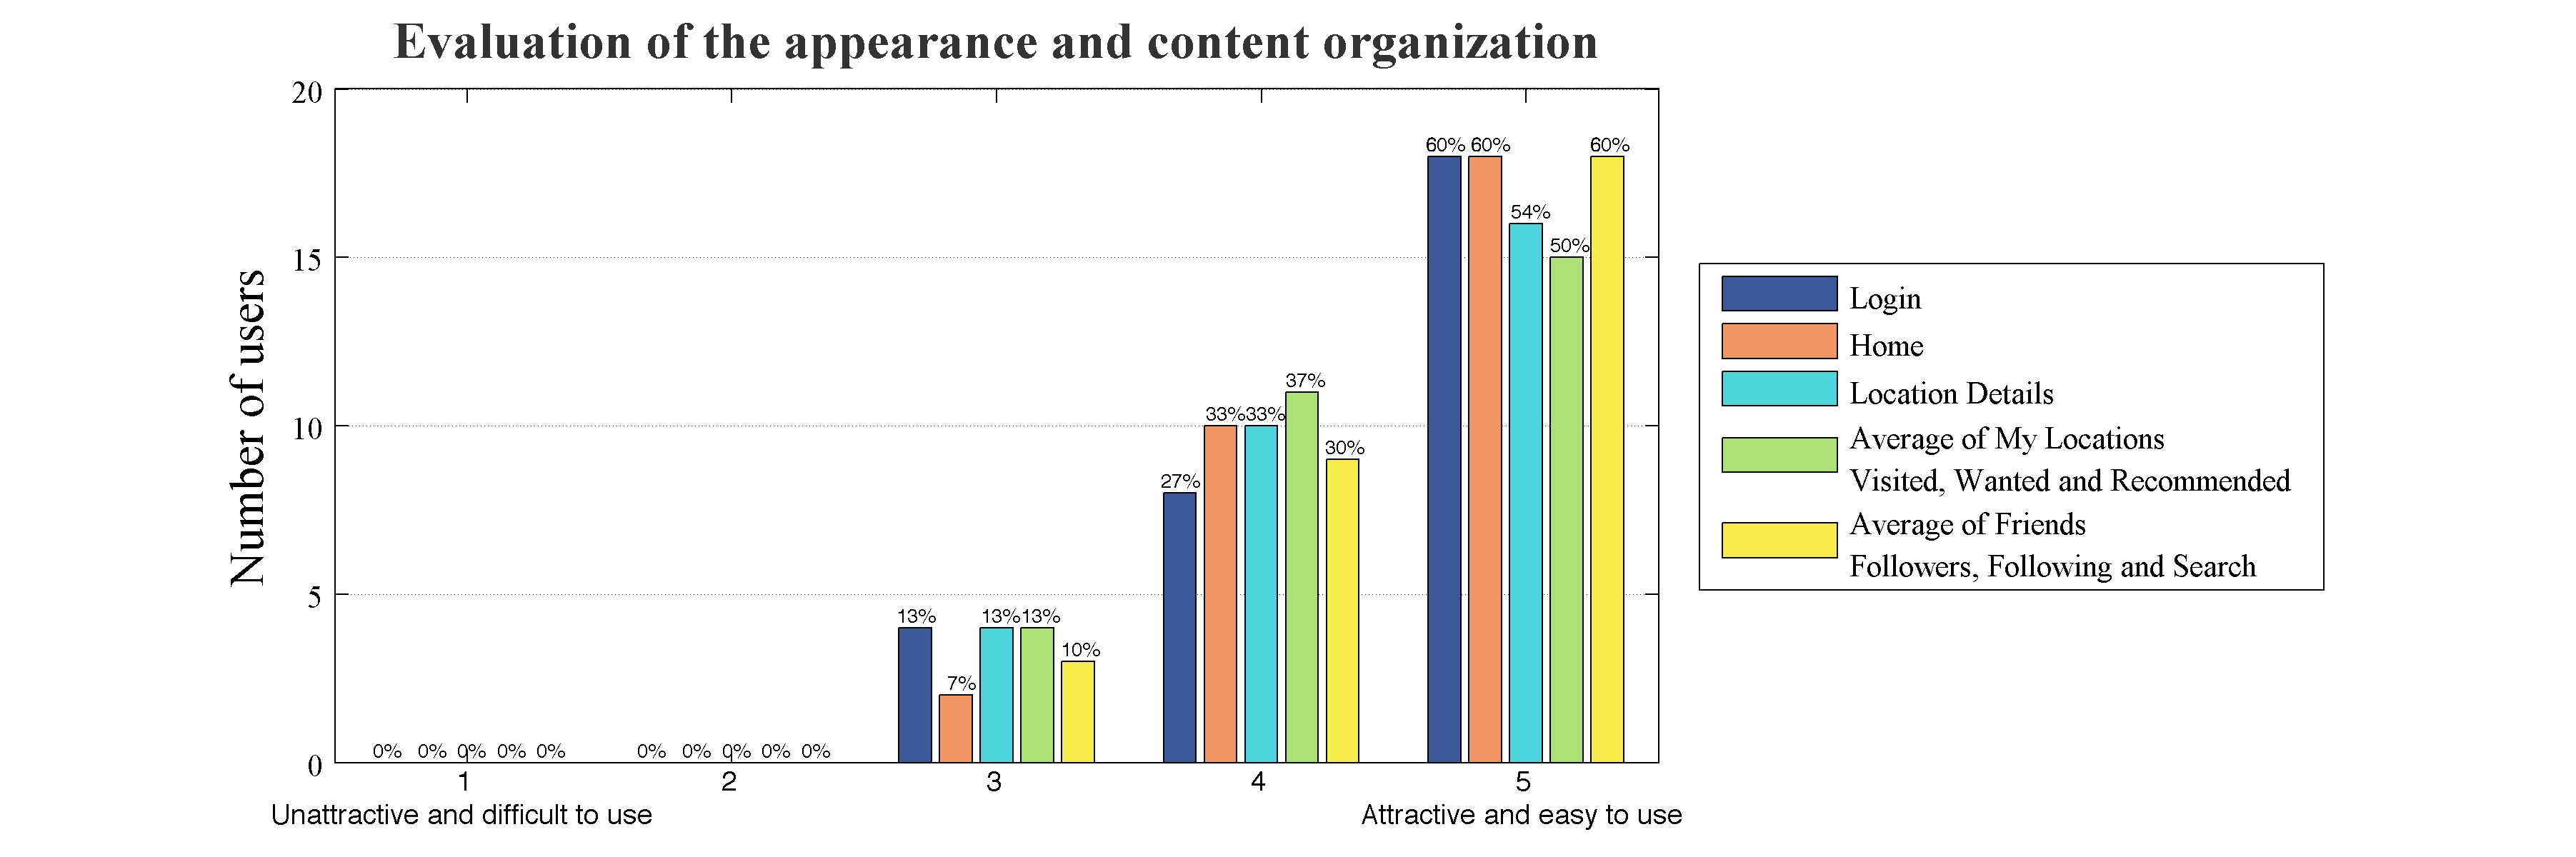
\includegraphics[width=16cm]{./images/charts/charts_eval_usability_and_appearence.jpg}
   \caption{Evaluation of the appearance and content organization.}
   \label{fig:usabilityOverall}
\end{figure}\\
%%%%%%%%%%%%
All screens share the similar rating distribution, where the majority of ratings are between 4 and 5, with a small group of users that have classified the screen with 3. The similar applies to the usefulness and importance of the available filters as well as the organization of the touristic location details screen, which evaluation is illustrated on Figure~\ref{fig:usabilityFeatures}.\\
%%%%%%%%%%%%
\begin{figure}[h!]
 \centering
   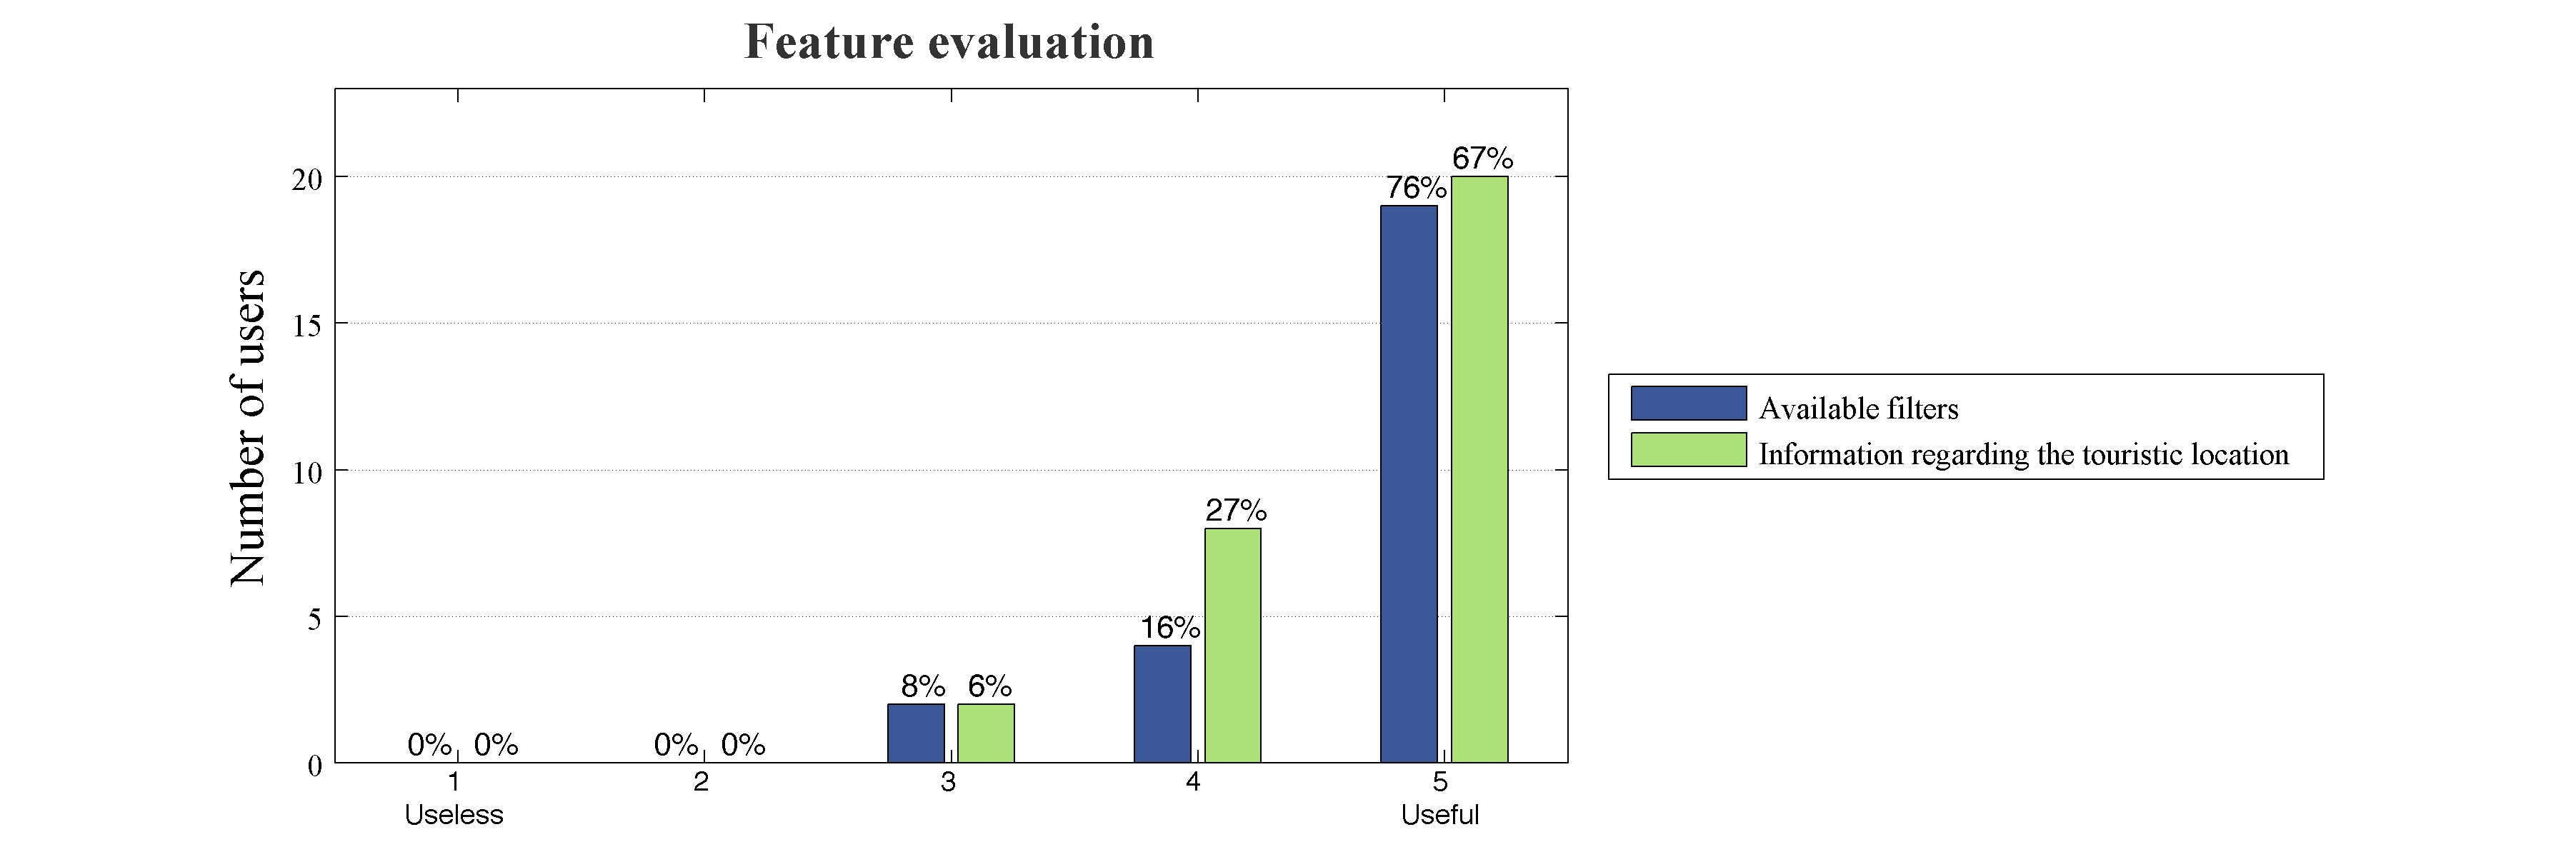
\includegraphics[width=16cm]{./images/charts/charts_eval_usability_features.jpg}
   \caption{Evaluation of the implemented features.}
   \label{fig:usabilityFeatures}
\end{figure}\\
%%%%%%%%%%%%
This analysis helped us to conclude that with the developed application we can reach the majority of users and provide them with an attractive and easy to use application for touristic assistance. On Figure~\ref{fig:usabilityInstallDistribution} is shown the distribution of the users that have answered \emph{Yes} and \emph{No} to the following question: \emph{In the future, would you install this app?}\\
%%%%%%%%%%%%
\begin{figure}[h!]
 \centering
   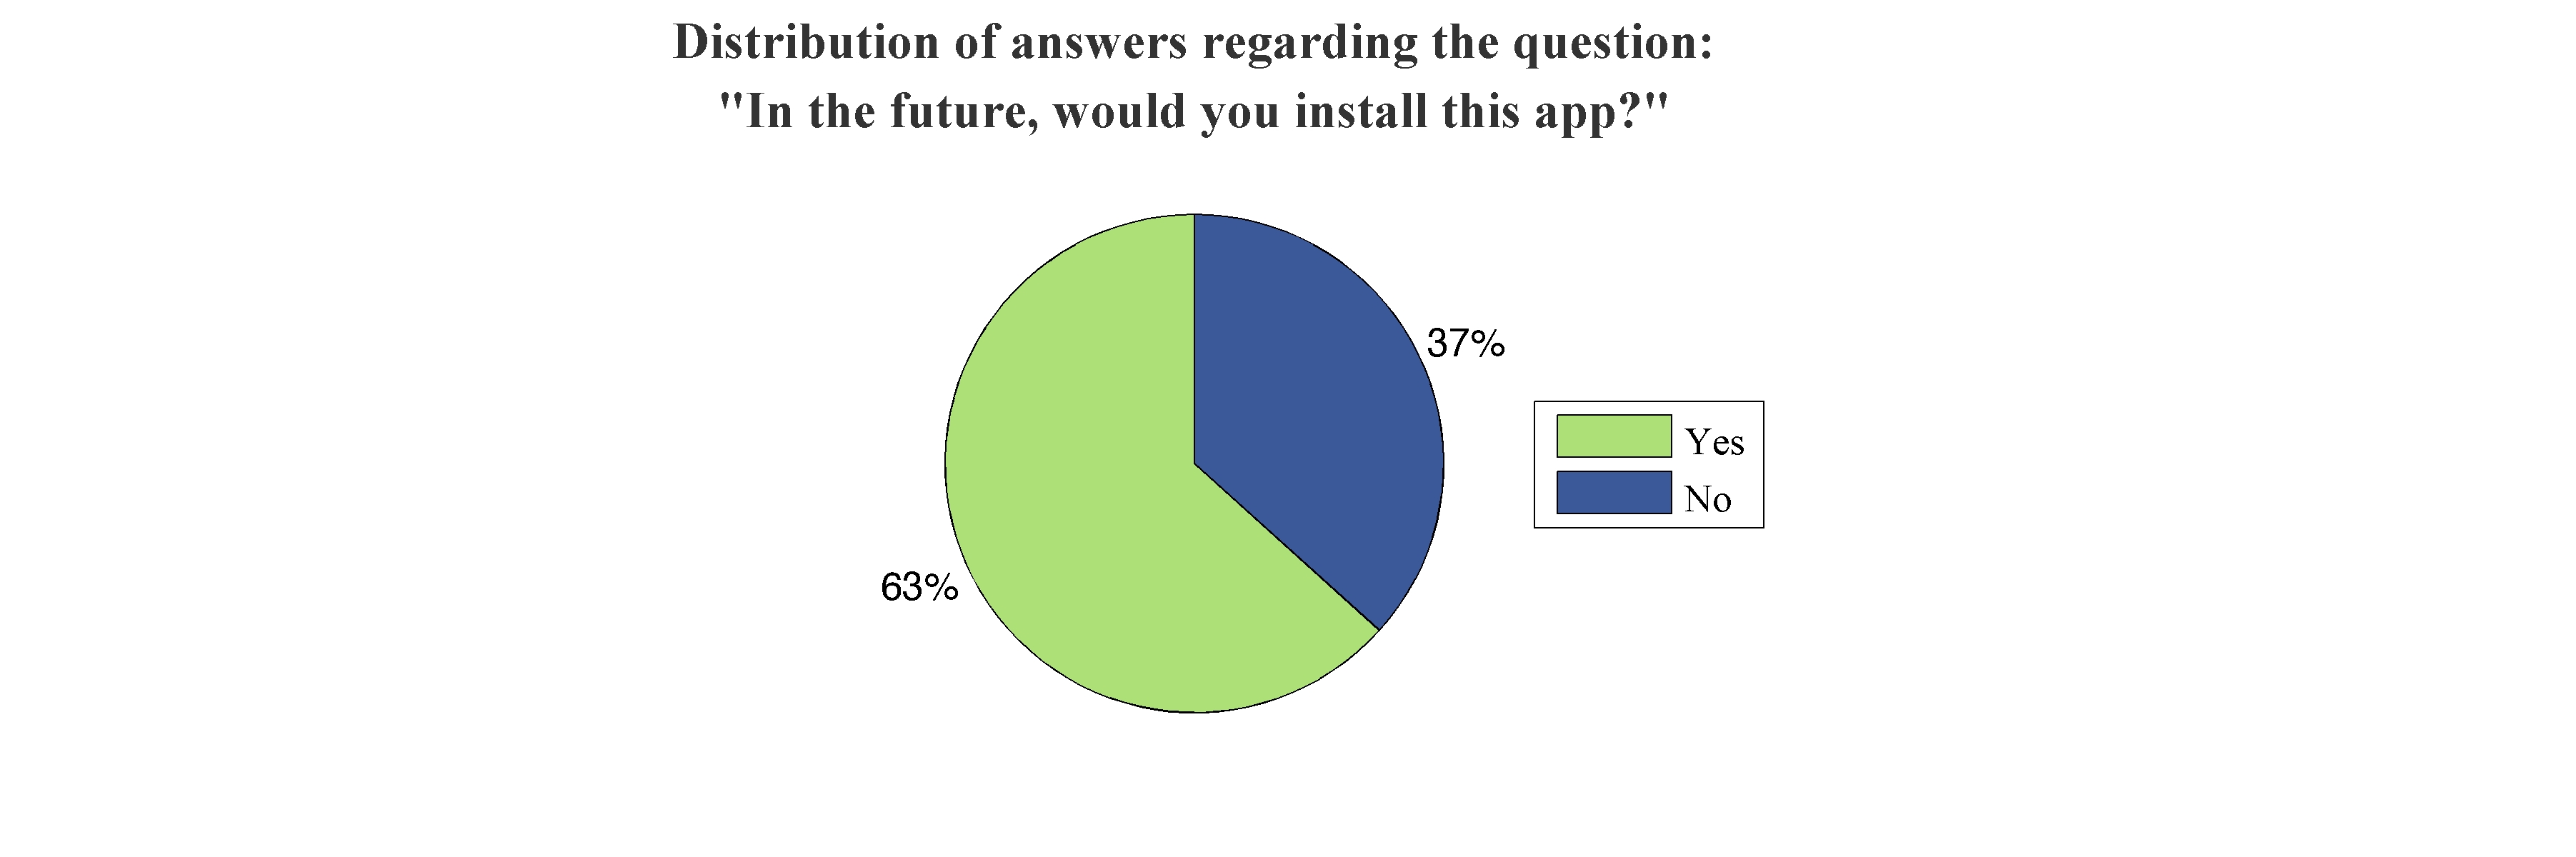
\includegraphics[width=16cm]{./images/charts/charts_eval_usability_will_install.jpg}
   \caption{Distribution of users that would like to install the application in the future.}
   \label{fig:usabilityInstallDistribution}
\end{figure}\\
%%%%%%%%%%%%
The majority have answered as \emph{Yes}. But, the people who have answered \emph{No}, have mostly answered to the questions 2.3 and 2.4 as follows:
\begin{itemize}
\item 2.3 How often are you using the external mobile applications?
	\begin{itemize}
		\item I have my set of favourite apps that I use regularly
		\item I rarely use external applications
	\end{itemize}
\item 2.4 Are you using any tourist guide application? 
\begin{itemize}
	\item No
	\item Yes, rarely
\end{itemize}
\end{itemize}
It is very difficult to achieve this type of users but they do not influence the evaluation of the application in a negative manner. The conducted evaluation has helped to understand our targeted audience and has ensured that the application is attractive and usable, with some interesting features to our users.